%%%%%%%%%%%%%%%%%%%%%%%%%%%%%%%%%%%%%%%%%%%% 80 line marker %%%%%%%%%%%%%%%

People in general are referring to this as the \emph{Information Age}. 
More and more data is available for each second that comes, and 
a vast amount of information passes us by every day. Yet, the demand for 
ways to collect data seem to only be increasing, this embodied in the new
wave of life-logging devices.

Our minds have not scaled along with this, so developing 
filters and making information searchable, shareable and observable
is a necessary mean for humans to process this data explosion. 

This is where Data Mining comes into the picture, by gathering qualitative
information from quantitative data. This master thesis will address Data Mining 
and Knowledge Discovery in small data sets produced by life-logging devices, 
first by clustering of spatial data to reduce dimensionality, then to classify 
these sets of objects by attaching tags or classes to them with semantic 
relevance.

\section{Motivation}

The project and thesis which this report describes has taken place 
at \emph{Narrative}\footnote{
    "Narrative is a young Swedish company with the ambition to give the 
    common man the opportunity of having a photographic memory. Our 
    specially designed camera takes two images per minute and our 
    cloud-based software and apps handles the sorting and managing of the 
    enormous amount of images for the user." - A translation of Narrative's 
    background in their description of the Master Thesis proposal. }
, a company which develops a life-logging, wearable camera. More general applications 
are of course of interest as well and will be pondered upon throughout the
report, but Narrative will be the primary example and the target for 
testing various data mining principles, as well as the source of quantitative
data. 

\subsection{Narrative}
As mentioned above, Narrative produces and sells a life-logging camera named
the \emph{Narrative Clip} (hereinafter referred to as the \emph{Clip})
which captures two images per minute along with sensor data from 
GPS\footnote{
    A \emph{Global Positioning System} sensor is fitted in the Clip, which 
    periodically listens for satellites and registers signal strength when
    possible. The position is then computed centrally, making the time stamp
    for the detection an error source, along with some in-accurateness of the 
    GPS signal in urban environments, as well as being completely unavailable
    indoors. 
}, Accelerometer\footnote{
    The accelerometer measures the force pulling the Clip towards the earth or 
    moving it in different directions. 
} and Magnetometer sensors\footnote{
    The magnetometer on the Clip measures the magnetic flow around the device,
    with the intention of providing a bearing of the camera lens, defined by
    the direction of the cross product of the accelerometer vector along with
    the magnetometer vector. However, this sensor is to sensitive to other
    sources of magnetism, often receiving a stronger field from a nearby 
    refrigerator than the magnetic pole, leaving this sensor too unreliable to
    be used.
}. The amount of data received by Narrative's cloud-based servers is huge, 
and hard to overview even for a single user with frequent usage of their device.

Enabling automatic classification of each image series (these specific image 
series are hereinafter referred to as \emph{Moments}, using Narrative's 
terminology) taken, makes each Moment more memorable, relateable and most 
importantly, more searchable for the customer. Narrative as a company 
can benefit from this as well, being able to answer questions such as \emph{
    "How many of our users use the Clip at home?" } 
and similar qualitative analysis questions not being possible to answer 
without reducing the quantity of the data. This type of answers are 
beneficial for instance in marketing, product evaluation, and self 
assessment of the company and the product.

Narrative is currently maintaining applications for different platforms
in order to view the Moments stored in their cloud. These platforms
currently consist of an Android app, an iOS app as well as a web
application. 

\subsection{Other Applications}
Looking in a broader perspective, this type of approach is 
of course applicable to similar social or informative services as well, 
but might also be useful in other areas. Wild animals monitored with tags 
that use low-frequency updates sensors is susceptible to a similar type of 
analysis, when for instance wanting to examine the sleeping behavior of a 
species, anomalies in individuals eating patterns and so on. The same goes 
for observing a group of team-working microrobots, analyzing if their 
behaviour is as expected, if some robots are malfunctioning or that the 
task in general is correctly performed \cite{discovering-moving-clusters}.

\section{Questions at Issue}

Given the background described above, questions regarding this arise. 
The focus of the resulting report as well as the project in general will 
revolve around these questions, and the project will aim for getting an 
answer to these questions.

\emph{ 
    What type of clustering algorithm is most suitable for data mining 
    in small data sets with few clusters? } 
    \refstepcounter{question}\thequestion\label{question:clustering}

The described motivation above, yields data sets which do not contain 
more than hundreds of spatial points. Detection of spatial clusters will 
enable a base for further knowledge discovery and classification of data 
series, and the same goes for the ability to detect the absence of 
clusters.

\emph{ 
    How well suited is Bayesian inference for deducting qualitative data 
    classifications in life-logging data sets, such as Narrative's 
    Moments? } \refstepcounter{question}\thequestion\label{question:bayes}

Given additional input apart from performed clustering, what else might be 
deductible, e.g. what classes might we assign a Moment given more stimuli 
than clustering? 

\section{Goal}
The goal of this thesis will be to answer the questions above by implementing a
proof-of-concept implementation built on Narrative's provided data set. 
%This report will revolve around this implementation, and algorithms as well
%as theory will be provided here that should be sufficient enough to 
%reproduce any results.

\subsection{Approach overview}
The Method chapter will provide a more in-depth description of the approach
and the methodology behind it. This section presents a short and comprehensive
introduction to how the questions in the previous section- will be answered.

For question~\ref{question:clustering} the idea is to implement and
evaluate representatives from different 
groups of algorithms on the basis of performance, quality and 
suitability. These algorithms are chosen from a spectrum of well-known 
implementations, with different approaches in order of get more diverse 
clustering approaches. Preferably three algorithms will be compared; one 
partitioning-based, one hierarchy-based, and one density-based (better 
explained in Approach). This is also closely related to how storage of the 
geographical points should be performed, the spatial data representation, 
which also is considered, as well as storage of detected clusters.

Regarding question~\ref{question:bayes}, \citeauthor{content-based-classification} 
has quite successfully analyzed images and assigned 
semantic classifications to said images based on Bayesian analysis. A similar 
approach should be applicable in this situation, delimited that 
probabilities and distributions will be assessed by educated guesses
\cite{content-based-classification, framework-classification}.
% , and training of the algorithm will be outside of the scope. 

\section{Technical Background}

\subsection{Clusters}

Mining quantitative data is closely related to the subject of clustering, 
as discovering clusters in a quantitative data set unravels  
qualitative information about the distribution of objects. This is a 
well-studied topic and has been for several decades at the point of 
writing this.

\subsubsection{Definition}

\citeauthor{why-so-many-clustering-algorithms}, author of 
\citetitle{why-so-many-clustering-algorithms},
argues that the notation of a cluster cannot be 
precisely defined, but rather that a cluster exists in the eye of the observer, which 
is one of the reasons why there are so many clustering algorithms 
\cite{why-so-many-clustering-algorithms}. A task that derives naturally 
from this is then to find a definition of a cluster that as many people as 
possible find satisfactory. There is no universal clustering algorithm 
because there is no universal definition of a cluster.

This of course means that in order to select a suitable clustering 
algorithm an analysis of what kind of clusters are to be detected 
needs to be done.

Another consequence of the indefinable concepts of clusters are that 
clustering algorithms in almost every case need some sort of knowledge 
about the data set to operate on, as what clustering is expected 
to be done. This is often represented as the need of input parameters
to the clustering algorithm, that defines how the algorithm will 
perform, and to some extent how a cluster is defined in that instance.

\subsection{Clustering algorithms}

As mentioned above, cluster discovery from data is a well-covered scientific 
topic where algorithms have been improved over the years. This report will 
focus on comparing different types of algorithms and to evaluate them based on 
a common evaluation method (later discussed). 

Clustering can be done on any type of data, of any dimensionality. The 
only prerequisite that is needed is a distance measurement that denotes
how similar or dissimilar two data points are. In this thesis, only 
spatial data is considered.

Classically, clustering algorithms are divided into three types: 
\begin{itemize}
    \item Partitioning Clustering Algorithms.
    \item Hierarchical Clustering Algorithms.
    \item Density-Based Clustering Algorithms.
\end{itemize}
all of which revolve around different ways to detect and to represent 
clusters. Other ways to divide clusters such as representative-based 
algorithms\footnote{
    Representative-Based algorithms use a single datum to represent each
    cluster, such as the Center Of Mass of the cluster or a 
    median representative. }
and model-based algorithms\footnote{
    Model-Based Algorithms use some sort of model to represent a 
    cluster, such as a polygon where some spatial objects are in the 
    center, and some in the cluster marginal. }
have been proposed as well, which is basically grouping the density-based 
and hierarchical algorithms together as they generally represent their 
clusters by models and not by medoids \cite{why-so-many-clustering-algorithms}.

\subsubsection{Partitioning Clustering Algorithms}

As the category name suggests, these algorithms partition the given 
spatial data in usually a predetermined number of clusters. Thus, traditional 
algorithms of this type often require knowledge
about how many clusters to partition the initial data set into, passed to 
the algorithm as a cluster parameter.

Partitioning algorithms are usually representative-based, and therefore
has difficulties recognizing non-convex clusters, since the COM (Center
Of Mass), or other representative, of a cluster might fall outside 
its bounds.

Examples of partitioning clustering algorithms are:
\begin{itemize}
    \item \emph{k-means clustering} partitions the input data set with 
        $n$ spatial objects into $k$ clusters, each cluster represented 
        by a mean spatial point. An arbitrary point $p$ belongs to 
        cluster $C$ represented by mean $m \in M$ if and only if 
        $d(p,m) = min_{m' \in M}{d(p,m')} $. $m \in M$ suggests that the
        k-means uses the above mentioned COM. The main cause for its 
        success and common use is its implementation simplicity, which
        is also the reason for the extensive amount of variations to 
        suit more specific needs. Some of these are variations are to 
        accommodate for the original problem's time complexity, as it 
        is NP-hard\footnote{
            NP-hardness denotes that the worst-case run-time of the 
            algorithm is not in polynomial time. Proof of this is 
            usually done by reduction of the problem to a problem that
            is known to be in NP.
        } even for small dimensions $d$ or a pre-determined number
        of clusters \cite{k-means-complexity}. When $k$ and $d$ is fixed,
        it can be solved in \ordo{n^{dk+1}\log{n}}. Relaxations to 
        increase efficiency of this scenario are also common \cite{k-means}.
    \item \emph{k-medoid clustering} essentially operates in the same 
        manner as k-means clustering, with the difference of actual 
        input objects (medoids) representing a cluster, instead of 
        the COM as k-means uses. One of the most common 
        implementations of this is PAM (Partitioning Around Medoids) 
        \cite{finding-groups-in-data}.
    \item \emph{CLARANS (Clustering Large Applications based on 
        RANdomized Search)} is inspired and motivated by PAM (as well as
        another algorithm presented by Kaufman \& Rousseeuw called 
        CLARA, Clustering LARge Applications 
        \cite{finding-groups-in-data}). Although both k-means and 
        k-medoids can be viewed as graph searches, CLARANS takes
        it one step further. Necessary input parameters are 
        $ numlocal $ - the number of local minima to visit and
        $ maxneighbour $ - the number of randomly selected 
        neighbours to visit in search of new local minima. As this 
        suggests, the algorithm is not optimal, but usually sufficient, 
        and more effective than CLARA, naive k-means and PAM \cite{CLARANS}.
\end{itemize}

\subsubsection{Hierarchical Clustering Algorithms}

Hierarchical Algorithms classify, or cluster, objects in an hierarchical manner 
rather than partitioning these spatial objects straight away, or base it on 
density-distribution.

These algorithms are usually divided into two sub-groups, \emph{agglomerative} 
and \emph{divisive} hierarchical clustering algorithms. The first
constructs the hierarchical structure of clusters (starting with combining 
spatial objects) bottom-up, while the latter one divides an all-covering 
cluster into several new ones. Then divisive flavor has also been seen 
conjunction with partitioning algorithms, where a distinction between the two 
sometimes is hard to do.

Hierarchical algorithms thus requires a termination condition to be 
defined, which determines when the merge or division process should be 
stopped. The difficulty here lies in deriving appropriate termination 
conditions, to make the algorithm perform clustering as desired.

Hierarchical algorithms naturally produce a dendrogram\footnote{
    A tree structure.
} of the clustered objects, since it involves either splitting or 
merging clusters on each step.

Examples of hierarchical clustering algorithms are:
\begin{itemize}
    \item \emph{SLINK} was meant as an improvement over classical
        agglomerative clustering, performing in $\mathcal{O}(n^2)$ instead
        of $\mathcal{O}(n^3)$ as the naïve agglomerative solution. This is 
        due to a different 
        pointer representation, and because of this the algorithm results
        in a dendrogram but no actual clusters. These have to be found 
        by specifying cutoff conditions to create the clusters \cite{SLINK}.
    %\item \emph{Ejcluster}
    %    \cite{Ejcluster}.
    \item \emph{Clusterpath} is a convex LP-relaxation of classical 
        hierarchical clustering algorithms, and needs the aid of a solver
        to perform clustering. A bonus of this relatively new method
        is that an object tree is obtained, which is cut in order to receive
        clusters \cite{clusterpath}.
\end{itemize}

\subsubsection{Density-Based Clustering Algorithms}
As the name suggests, density-based clustering algorithms base their
clustering on the density of data, and can recognize clusters of 
arbitrary shape. Most density-based algorithms are based on a grid and 
sensitive to the settings of this grid which heavily affects the clustering 
results. How this grid is set up can be viewed as the clustering algorithm 
input parameters, which as previously mentioned is a necessity for most
clustering algorithms.

These algorithms are often model-based, and are therefore applicable to 
more arbitrarily-shaped clusters. A still remaining  problem is the
difficulty to detect clusters of various density, since input parameters 
often control these clustering factors for density-based algorithms.

Examples of density-based clustering algorithms are:
\begin{itemize}
    \item \emph{DBSCAN (Density Based Spatial Clustering of Applications 
        with Noise)} is an algorithm that is not based on any grid, but 
        instead the notation of the neighbourhood of a point, and the 
        separation of border points and core points of a cluster. The 
        core point criterion 
        (definition \ref{definition:directly-density-reachable})
        is essential when defining which data can be regarded as being
        core points, and which will be classified as border points of a
        cluster. This algorithm also disregards noise, if any data diverges
        too much from the rest of the set \cite{DBSCAN}.
    \item \emph{OPTICS (Ordering Points To Identify the Clustering Structure)} 
        is not strictly a clustering algorithm per se, since it does not 
        perform any clustering in itself.
        Motivated by some shortcomings of DBSCAN (regarding difficulties of 
        detecting clusters of varying densities), the input spatial
        data is sorted in a manner to make clustering afterwards easier,
        but leaves the clustering to other implementations.
        OPTICS requires the same input as DBSCAN, but is less sensitive 
        to the parameter values \cite{OPTICS}.
\end{itemize}

\subsection{Evaluation}
As mentioned above, a cluster only exists in the eyes of the 
beholder. That means, when it comes to evaluation of an algorithm 
performance it is not clear how to compute whether the algorithm has produced
correct clusters or not, since there is no definition of a correct clustering solution. 
\begin{figure}[h!]
    \centering
    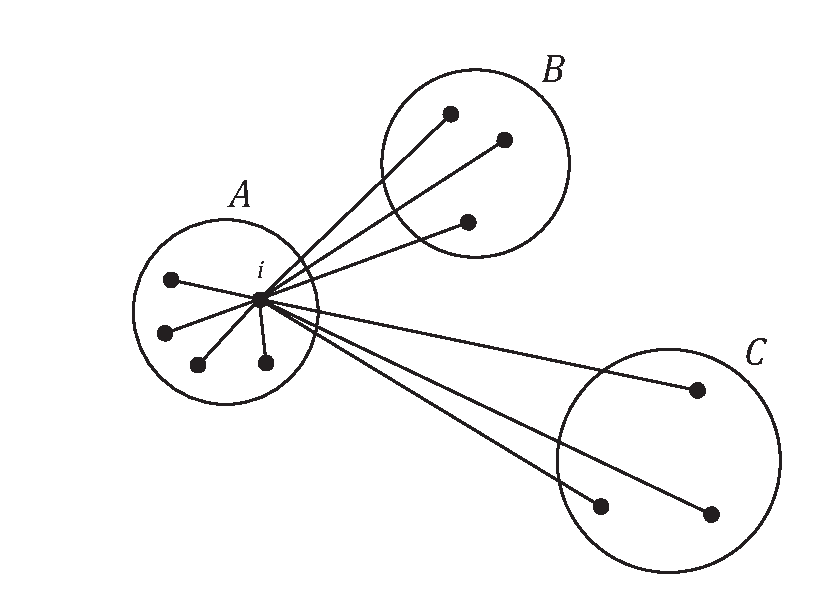
\includegraphics[width=0.5\textwidth]{images/silhouette_computation_clusters.pdf}
    \caption{Silhouette computation example for a single data point.
    \label{fig:silhouette-computation-clusters} }
\end{figure}

Therefore \citeauthor{silhouettes}, author of \citetitle{silhouettes}, speaks of detected clusters
as artificial or natural, based on visual inspection, and proceeds 
to introduce \emph{Silhouettes} as a graphical aid for detecting 
such artificial fusions of data. The silhouette of a data point is 
denoted by a numerical value in the interval $[-1, 1]$, denoting how well
the particular data point belongs to the cluster it is currently
assigned to. A higher value indicates a better assignment.

Silhouettes are, somewhat simplified, defined by dividing the mean
distance from the point of concern (in 
figure~\ref{fig:silhouette-computation-clusters} denoted by $i$) to
all other points in the same cluster $A$, with the mean distance from
$i$ to all points in the nearest not assigned cluster, $B$. The following
equation shows the computation process:
\begin{equation}
    \label{eq:silhouette-computation}
    s(i) = \frac{b(i) - a(i)}{\max\{a(i), b(i)\}}
\end{equation}
where $i$ is the point of concern, $a(i)$ is the average distance
from $i$ to all other points in $A$, and $b(i)$ is the average
distance from $i$ to all points in $B$.

Silhouettes were suggested to be visualized by a 
horizontal bar plot, each bar denoting the silhouette value of 
each point in the cluster the point was assigned to. 

Given that, it is desirable to have wide silhouettes describing the
clusters, and that the silhouettes should be even edged. A mean 
silhouette width $ \bar{s} $ can also be computed, in order of 
giving condensed, numerical interpretation of how natural the 
clustering is of a processed data set \cite{silhouettes}.

In a later work \citeauthor{finding-groups-in-data} suggests using
a \emph{Silhouette Coefficient} ($ SC $), that is the maximum 
$ \bar{s}(k) $ over various $ k $ using a partitioning clustering 
method
\begin{equation}
    \label{eq:silhouette_coefficient}
    SC = \max_{ k } \bar{s}(k)
\end{equation}
which suggests how well the data set is suitable for clustering 
given the particular clustering method being used.
Table \ref{table:silhouette-interpretation} provides a suggested
interpretation of the silhouette coefficient, as provided by
\citeauthor{finding-groups-in-data} \cite{finding-groups-in-data}.

\begin{table}
    \centering
    {\begin{tabular}{ | l | l | }
        \hline
        SC & Proposed interpretation \\
        \hline
        0.71 - 1.00 & A strong structure has been found.\\
        0.51 - 0.70 & A reasonable structure has been found.\\
        0.26 - 0.50 & The structure is weak and could be 
                      artificial.\\
        $<$    0.26 & No substantial structure has been found.\\
        \hline
    \end{tabular}}
    \caption{Silhouette Coefficient interpretation.} 
    \label{table:silhouette-interpretation}
\end{table}

If one considers table \ref{table:silhouette-interpretation} 
from a $ \bar{s} $ point of view instead of $ SC $, this should 
be applicable for determining the quality of found clusters by 
an arbitrary algorithm.

It is notable that silhouettes are not meaningful when clustering 
algorithms produce a single cluster, since the definition of a 
silhouette describes the relation of points similarity to its 
assigned cluster and the closest cluster which it is not assigned
to, which will not exist given that there is only one cluster. 
\citeauthor{silhouettes} suggests assigning this sort of
silhouette a value of 0 for comparison reasons, as this is the 
most neutral value. 

\subsection{Data Representation}
A sound way of representing detected clusters is necessary, in 
order not to have to re-run the clustering algorithms each 
time a knowledge discovery is requested. Being able to position 
clusters and use knowledge about previously recorded clusters is
another necessity, to make the algorithm learn based on user
corrections (of for instance the name of locations). 
After all, the sought result is to classify Moments
and clusters with \emph{semantically significant} and
\emph{meaningful} names, and 
being corrected by a user on a cluster name should trump 
everything else, thus being more significant. Detected clusters
at the same position as a previous should have the same name, not
only for being as correct as possible, but also in order 
not to be ambiguous in classified cluster names. 

Many databases today support geo-spatial queries for both points and
polygons\footnote{
    Here, only 2-dimensional data is considered which is the most 
    commonly supported, although support for 3-dimensial data exist
    in many database solutions.
}, and in this case it is the latter that is of interest. 
Being able to store clusters as areas, and persist these areas 
represented as polygons enable another level of detection for 
clusters, where it is possible to detect if it is a cluster that 
is known previously. Queries asking for overlapping clusters are
in general supported by 
\emph{Spatial Database Management Systems} (SDBMS) using 
\emph{Dimensionally Extended Nine-Intersection Model} 
DE-9IM\footnote{
    DE-9IM is a model for representing spatial relationships 
    between polygons and geo-spatial shapes. This is defined
    by a matrix specifying Interior, Boundary and Exterior 
    attributes between the different shapes, and varying 
    configuration of the resulting matrix is interpreted as
    spatial relationships such as \emph{Touches}, \emph{Disjoint},
    \emph{Equals} etc \cite{DE-9IM}. }

The support for performing geo-spatial queries on a database and 
doing this efficiently is usually implemented with some sort of 
\emph{spatial index}. Common implementations are R-trees 
and R*-trees, which fits the spatial entities into rectangles of
varying sizes in a tree structure, allowing a lookup time of 
\ordo{log(n)}, by balancing the trees \cite{R-trees, R*-trees}.

Apart from storing polygons, it is useful during this paper to
also persist the spatial points which make the cluster. This is 
for evaluation purposes, as algorithms examining the quality or
naturalness of a cluster in general needs access to all the points
in the particular cluster.

\subsubsection{RethinkDB}
RethinkDB will be used in the sought proof-of-concept implementation,
as it fulfills the necessary requirements, with support for spatial
queries and storage of spatial data both as geographical points, and
polygons.

It is an Open Source project hosted on GitHub, and has a growing 
community at the time of writing providing support when needed. Narrative
is currently using RethinkDB as a cache-layer for API requests, making
it an even stronger candidate for the proof-of-concept implementation.

\section{Classification}
Classification of data is closely related to clustering of data, 
and the two problems are not even distinguishable in all 
applications. 

\subsection{Bayesian Inference}

Bayesian inference is a methodology for updating beliefs about a model
when certain evidence is observed, while preserving some level of 
uncertainty.

The entry point is some \emph{Prior probability} $Pr(\theta)$ that the model 
we are observing is in world $\theta$. There exist \emph{likelihoods} 
$ Pr(x_i|\theta) $ that some \emph{evidence} $ x_i $ will be observed in
this $\theta$ world. Given this framework, the target is often to 
compute a \emph{Posterior probability} containing updated beliefs about
the state of the world provided the witnessed evidence. 

A model representing Bayesian beliefs can easily be graphically 
interpreted as a \emph{Bayesian Network}. Bayesian networks are Probability 
DAG:s (\emph{Directed Acyclic Graphs}), and are used for modeling the 
probability of certain events when other events are known. 

%% HERE

In this report, a Bayesian network is used to model the probability of a 
series of positions (or more exactly, photographs with positions attached)
enhanced with additional sensor data belonging to a certain class.

As this introduction previously established that expected results from 
clustering algorithm are not precisely defined and lies in the eyes of 
the beholder. If the results are somewhat fuzzy, and somehow can be 
computationally evaluated according to some metric, this should prove as 
a suitable parameter for an automatic decision algorithm, such as one 
powered by a Bayesian network, which is the idea behind the implementation
that is described. 

Bayesian networks are the base for Bayesian analysis, which starts with
a prior probability $ Pr(\theta) $ and a likelihood given $ Pr(x_i|\theta) $
in order to compute a posterior probability $ Pr(\theta|x_j) $. In the case
of this report, $ x_i $ represents some input probability while $ x_j $
represents some class or end condition.

With each inferred parameter, a dimension is added to the state-space\footnote{
    The state-space is defined as the possible states for a world to be in, and
    increases with each dimension added.
}. This makes high-dimensional models hard to observe and analyze by inspection, 
since modelling more then 3 or perhaps 4-dimensional probability space of 
various parameters is not possible to visualize. 

\subsubsection{Fitting of models}
As models become complex when inferring high dimensionality and observing
evidence (thus forcing other probabilities in the model to alter), 
visualization of the probability of a certain unobserved variable becomes
harder. Simply outputting some mathematical formula is not intuitively
graspable and computing such a formula is usually hard or impossible when other 
parameters have been described by sample data.
%and not by mathematical probability functions. 

\emph{Markov Chain Monte Carlo (MCMC)} are a category of algorithms 
dealing with this particular matter, and instead describes the probability
of theses parameters using thousands of samples. The main target is to 
cover as much of the state-space as possible by randomly drawing samples
in a manner that makes the returned collection as close to the true 
distribution as possible. 

When a fitting algorithm is proven to approach the true underlying 
distribution, when provided with enough steps and enough samples, it is 
denoted that the algorithm \emph{converges}. 

\subsubsection{PyMC}
\emph{PyMC} is the framework used for Bayesian modeling of the
classification problems in this report. PyMC:s online user manual
states:

\blockquote{
    ``PyMC is a python module that implements Bayesian statistical 
    models and fitting algorithms, including Markov chain Monte Carlo. 
    Its flexibility and extensibility make it applicable to a large 
    suite of problems. Along with core sampling functionality, 
    PyMC includes methods for summarizing output, plotting, 
    goodness-of-fit and convergence diagnostics.''
    - PyMC User's Manual \cite{pymc}.}

PyMC fits the needs of this project well, as it implements the
core functionality necessary for Bayesian inference such as a range
of probability functions as well as fitting algorithms, mainly MCMC.
%(in particular, a flavor of MCMC called INSERT HERE)
It is also 
bundled with algorithms for finding an appropriate starting point for
the fitting algorithms to work with, as this affects the rate of 
convergence for the fitting algorithm.

\section{Limitations}

\subsection{Image analysis}
Only very simple and limited image analysis is applied in this 
report, as this could easily have made subject for a thesis of 
its own (as is the case with other reports) 
\cite{content-based-classification, framework-classification}. 

The purpose of this thesis is not classification of images as
such, but of small series of data samples of varying length. 

\subsection{Individual classification}
Interesting as it might be with performing individual 
classification of data, in this case images, this is deemed
outside of scope for this report, due to time limitations. 

The subject considered is, as mentioned above, deducting 
information about a data set as a whole given attributes in 
separate data.

\subsection{Automatic Learning of Network structure}
In machine learning there exist a lot of literature about the
subject of automatically determining network structure of 
a Bayesian network, opposed to let it be specified by an
expert. The intent is here to describe the automated process
of data set classification, and the initial step such as 
setting up the decision network is assumed to be done. For 
simplicity reasons, the second approach is chosen, and 
extending the work later on by learning the network structure
computationally does not interfere with the work of this 
report.

\subsection{Exact Probabilities}
Exact distributions of probabilities of events are hard to 
come by, and are by its nature virtually impossible to 
confirm (given that it is probabilities). This report will not
focus on determining these optimally, but rather leave the 
estimated distributions to be decided based on a bit of logical
reasoning. 

\subsection{Semantic Significance}
Choosing labels for derived classes is a problem of its own, and
will not to its full extent be discussed in this report. As 
\citeauthor{content-based-classification}, authors of 
papers~\citetitle{framework-classification} 
and~\citetitle{content-based-classification},
% Would like to reference both, but it is the same author, 
% "framework-classification"
mentions, search queries often describe more high-level attributes
about data sets, or images in this case, such as a search would more
likely consist of the word "sunrise" when looking for an image, than
"predominantly red and orange" 
\cite{framework-classification, content-based-classification}.

The semantic significance of the label of a class can therefore 
describe how meaningful that label is, although assessing in full 
scale how significant the labels are in this report will be left 
for future research.
\subsection{Only 2-dimensional spatial data is considered}
One might consider data of higher dimensionality, encountering
other problems than the spatial clustering in this thesis report.
This will however not be done here, as this does not seem to
have enough relevance for this case. 

\section{Related Work}
\citetitle{finding-groups-in-data} by 
\citeauthor{finding-groups-in-data} is regarded by many as the 
classic text-book in cluster analysis which provides and 
introduces several theories that prove the foundation of 
cluster theory today \cite{finding-groups-in-data}.
\citeauthor{silhouettes} is also the author of the 
paper~\cite{silhouettes}, that introduces a universal way of 
evaluating clustering performance under certain conditions, such 
as that the number of clusters has to be greater than 1. This 
method is used in this thesis and is discussed itself, based on 
its suitability to accommodate for different clustering solutions.

Article~\cite{why-so-many-clustering-algorithms} is a position 
paper describing ways of looking at clusters and cluster analysis 
on a broad spectrum, and explains the difficulties as well as 
why there is no universal solution to clustering. 

The papers~\cite{DBSCAN, OPTICS, CLARANS, Ejcluster, SLINK, clusterpath, k-means, finding-groups-in-data} 
all describe various clustering algorithms used and were considered 
as prospects for evaluation in this thesis. 

Papers~\cite{R-trees, R*-trees} both describe ways of implementing 
spatial indexes, which are the core of a spatial data base and making 
spatial queries possible in an efficient manner. 

The article~\citetitle{P-DBSCAN} at first glance seem to be very similar in 
its aim as this this, but the difference lies in intention. While 
\citeauthor{P-DBSCAN} tries to deduct information about attractive
areas and places using clustering of photographs, the approach of this 
paper is to deduct information about a series of photos using areas 
and places. \cite{P-DBSCAN}

The paper~\cite{bayesian-class-gauss-proc} introduces learning of detection of 
probabilities modeled by Gaussian Processes by interpreting the 
classification as a regression problem. This allows small training 
sets, which Bayesian numerical techniques for calculating the trace 
and determinant was not as tolerant of. 

Papers~\cite{content-based-classification, framework-classification} use a
Bayesian approach for classifying individual images based on their 
visual attributes, which is fairly closely related to this work. This
provides interesting results inspiring this thesis, with the difference
of classifying series of images instead of single images, and choosing
other attributes to base the classification on.

\cite{bayesian-methods-for-hackers} explains thoroughly how one might
regard Bayesian inference and methods from a programming perspective 
with examples in PyMC, rather than using traditional mathematical notation
to address the problems. 
(Not clear if this is a valid resource, but it sure was helpful).
Similarly, \cite{bayesian-theory} provides more in-depth foundation
with weight distributed on the theoretical parts of Bayesian 
analysis.

\cite{the-most-dangerous-equation} explains the pitfalls of de Moivres 
equation by reciting some statistical mishaps throughout history. This 
explains the care one has to take to not draw premature conclusions from
small data sets. 

% Re-read
\cite{discovering-moving-clusters} describes discovery moving of spatial 
clusters, and thus introduces another dimension into the clustering; time.
This is similar to the approach suggested in this thesis, with the 
difference of observing a lot of spatial points at once. 

\cite{hierarchical-evaluation} discusses and compares different 
methods of evaluation hierarchical clustering algorithms. 

\cite{twitter-geo} is an example of a real-time, big data application 
using spatial content in the social network Twitter to locate events
on a map, similar

Article~\cite{iphone-wifi} evaluates the accurateness of mobile units 
with regard to GPS data, and different techniques that can be used for 
obtaining this in an urban area. This is useful to keep in mind, as 
a similar implementation for life-logging devices and the Clip lies 
close in the future.

\section{Report Structure}

This section has presented the motivation and technical foundation
for the work done in this paper. More specific implementation 
details and theory will be addressed in chapter \ref{ch:method}.
The results of these implementations will be presented with 
measured test data in chapter \ref{ch:result}. These results 
will later be evaluated and discussed under chapter 
\ref{ch:discussion}, as well as other factors that might have 
influenced the results. Finally, a conclusion is drawn in chapter 
\ref{ch:conclusion} as well as suggestions for further research 
on the subject.

The appendices contain further implementation details beyond what
is described in the report. These should not be necessary to grasp
the main outlines of the report, but prove interesting for a full
understanding of how algorithms have been implemented in this work.